\chapter{Introducción}
\chapterquote{Tortugas quote}{Autor}

\section{Opciones que acepta el estilo}
\label{S:opciones-que-acepta}

La mayoría de las especies animales son capaces de realizar complejos patrones de movimientos que generalmente dependen del ambiente, factores intrínsecos de los individuos y las interacciones entre ellos (\cite{morales2005adaptive}, \cite{morales2010building} y \cite{nathan2008emerging}). La complejidad de estos movimientos están manifestados en sus trayectorias. Para el caso de las tortugas estas trayectorias dependen fuertemente de la vegetación en la zona de estudio y la época del año (caso que busquen reproducirse, depositar sus huevos, etc.).


Nuestra especie de interés es la tortuga $Chelonoidis$ $chilensis$. Se distribuye desde el Gran Chaco hasta el norte de la Patagonia, como se muestra en la Fig.~\ref{fig:distribuciondeEspecie} (\cite{chebez2008se}). Esta especie está incluida en el Appendix  de la \textit{Convention on International Trade in Endangered Species of Wild Fauna and Flora (CITES)} y fue categorizada como \textit{vulnerable} a nivel nacional \cite{prado2012categorizacion} e internacional por la \textit{International Union for Conservation of Nature (IUCN)}.
Los principales factores que llevaron a esta situación son la reducción, modificación y destrucción de su hábitat, debido a la expansión de la frontera agropecuaria, y su comercialización, siendo la especie nativa de reptiles más ilegalmente traficada en el mercado de mascotas en Argentina (\cite{prado2012categorizacion}). Además, la amenaza a esta especie se ve aumentada con la introducción de especies depredadoras exóticas como el Jabalí (\textit{Sus scrofa}) (\cite{kubisch2014chelonoidis}). En este trabajo estudiaremos una población de tortugas en en el límite sur de su distribución geográfica, a 20 km al norte de San Antonio Oeste, provincia de Río Negro.  \\
    
Las tortugas son animales  herbívoros que se alimentan con tallos y frutos de cactus (\textit{Opuntia sulphurea, Cereus aethiops, Perocactus tuberosus}), gramíneas (\textit{Chloris castilloniana, Trhichloris crinita}), herbáceas (\textit{Alternanthera pugens, Sphaeralcea miniata, S. mendocina, Portulaca grandiflora}) y vainas de leguminosas (\cite{zacarias2016biologia}).
    
    
    
\begin{figure}[h]
    \begin{center}
        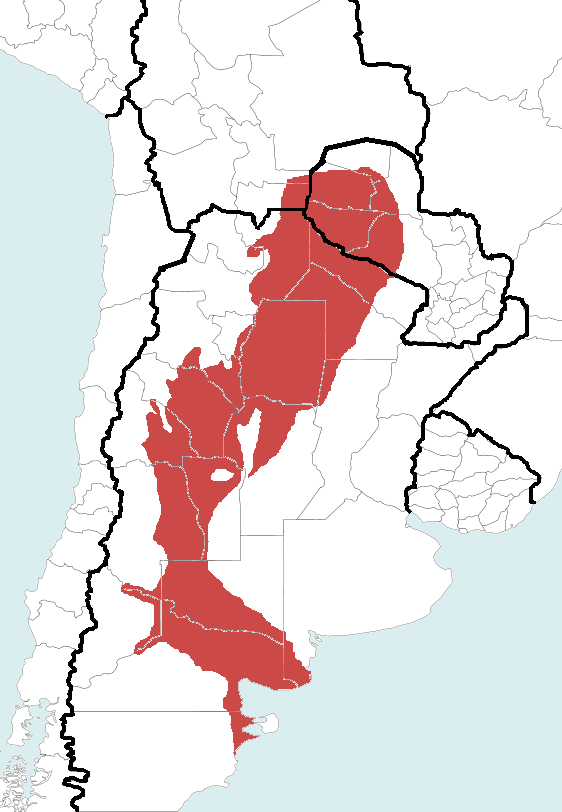
\includegraphics[width=\imsize]{figs/Chap1/Chelonoidis_chilensis_geographic_range.png}
        \caption{Distribución geográfica de la especie de tortuga \textit{Chelonoidis chilensis} \label{fig:distribuciondeEspecie}.}
        
        \end{center}
\end{figure}

%%% Local Variables: 
%%% mode: latex
%%% TeX-master: "template"
%%% End: 
